% Options for packages loaded elsewhere
% Options for packages loaded elsewhere
\PassOptionsToPackage{unicode}{hyperref}
\PassOptionsToPackage{hyphens}{url}
%
\documentclass[
  letterpaper,
  oneside,
  openany]{scrbook}
\usepackage{xcolor}
\usepackage[lmargin=1in,rmargin=1in,tmargin=1in,bmargin=1in]{geometry}
\usepackage{amsmath,amssymb}
\setcounter{secnumdepth}{5}
\usepackage{iftex}
\ifPDFTeX
  \usepackage[T1]{fontenc}
  \usepackage[utf8]{inputenc}
  \usepackage{textcomp} % provide euro and other symbols
\else % if luatex or xetex
  \usepackage{unicode-math} % this also loads fontspec
  \defaultfontfeatures{Scale=MatchLowercase}
  \defaultfontfeatures[\rmfamily]{Ligatures=TeX,Scale=1}
\fi
\usepackage{lmodern}
\ifPDFTeX\else
  % xetex/luatex font selection
\fi
% Use upquote if available, for straight quotes in verbatim environments
\IfFileExists{upquote.sty}{\usepackage{upquote}}{}
\IfFileExists{microtype.sty}{% use microtype if available
  \usepackage[]{microtype}
  \UseMicrotypeSet[protrusion]{basicmath} % disable protrusion for tt fonts
}{}
\makeatletter
\@ifundefined{KOMAClassName}{% if non-KOMA class
  \IfFileExists{parskip.sty}{%
    \usepackage{parskip}
  }{% else
    \setlength{\parindent}{0pt}
    \setlength{\parskip}{6pt plus 2pt minus 1pt}}
}{% if KOMA class
  \KOMAoptions{parskip=half}}
\makeatother
% Make \paragraph and \subparagraph free-standing
\makeatletter
\ifx\paragraph\undefined\else
  \let\oldparagraph\paragraph
  \renewcommand{\paragraph}{
    \@ifstar
      \xxxParagraphStar
      \xxxParagraphNoStar
  }
  \newcommand{\xxxParagraphStar}[1]{\oldparagraph*{#1}\mbox{}}
  \newcommand{\xxxParagraphNoStar}[1]{\oldparagraph{#1}\mbox{}}
\fi
\ifx\subparagraph\undefined\else
  \let\oldsubparagraph\subparagraph
  \renewcommand{\subparagraph}{
    \@ifstar
      \xxxSubParagraphStar
      \xxxSubParagraphNoStar
  }
  \newcommand{\xxxSubParagraphStar}[1]{\oldsubparagraph*{#1}\mbox{}}
  \newcommand{\xxxSubParagraphNoStar}[1]{\oldsubparagraph{#1}\mbox{}}
\fi
\makeatother

\usepackage{color}
\usepackage{fancyvrb}
\newcommand{\VerbBar}{|}
\newcommand{\VERB}{\Verb[commandchars=\\\{\}]}
\DefineVerbatimEnvironment{Highlighting}{Verbatim}{commandchars=\\\{\}}
% Add ',fontsize=\small' for more characters per line
\usepackage{framed}
\definecolor{shadecolor}{RGB}{241,243,245}
\newenvironment{Shaded}{\begin{snugshade}}{\end{snugshade}}
\newcommand{\AlertTok}[1]{\textcolor[rgb]{0.68,0.00,0.00}{#1}}
\newcommand{\AnnotationTok}[1]{\textcolor[rgb]{0.37,0.37,0.37}{#1}}
\newcommand{\AttributeTok}[1]{\textcolor[rgb]{0.40,0.45,0.13}{#1}}
\newcommand{\BaseNTok}[1]{\textcolor[rgb]{0.68,0.00,0.00}{#1}}
\newcommand{\BuiltInTok}[1]{\textcolor[rgb]{0.00,0.23,0.31}{#1}}
\newcommand{\CharTok}[1]{\textcolor[rgb]{0.13,0.47,0.30}{#1}}
\newcommand{\CommentTok}[1]{\textcolor[rgb]{0.37,0.37,0.37}{#1}}
\newcommand{\CommentVarTok}[1]{\textcolor[rgb]{0.37,0.37,0.37}{\textit{#1}}}
\newcommand{\ConstantTok}[1]{\textcolor[rgb]{0.56,0.35,0.01}{#1}}
\newcommand{\ControlFlowTok}[1]{\textcolor[rgb]{0.00,0.23,0.31}{\textbf{#1}}}
\newcommand{\DataTypeTok}[1]{\textcolor[rgb]{0.68,0.00,0.00}{#1}}
\newcommand{\DecValTok}[1]{\textcolor[rgb]{0.68,0.00,0.00}{#1}}
\newcommand{\DocumentationTok}[1]{\textcolor[rgb]{0.37,0.37,0.37}{\textit{#1}}}
\newcommand{\ErrorTok}[1]{\textcolor[rgb]{0.68,0.00,0.00}{#1}}
\newcommand{\ExtensionTok}[1]{\textcolor[rgb]{0.00,0.23,0.31}{#1}}
\newcommand{\FloatTok}[1]{\textcolor[rgb]{0.68,0.00,0.00}{#1}}
\newcommand{\FunctionTok}[1]{\textcolor[rgb]{0.28,0.35,0.67}{#1}}
\newcommand{\ImportTok}[1]{\textcolor[rgb]{0.00,0.46,0.62}{#1}}
\newcommand{\InformationTok}[1]{\textcolor[rgb]{0.37,0.37,0.37}{#1}}
\newcommand{\KeywordTok}[1]{\textcolor[rgb]{0.00,0.23,0.31}{\textbf{#1}}}
\newcommand{\NormalTok}[1]{\textcolor[rgb]{0.00,0.23,0.31}{#1}}
\newcommand{\OperatorTok}[1]{\textcolor[rgb]{0.37,0.37,0.37}{#1}}
\newcommand{\OtherTok}[1]{\textcolor[rgb]{0.00,0.23,0.31}{#1}}
\newcommand{\PreprocessorTok}[1]{\textcolor[rgb]{0.68,0.00,0.00}{#1}}
\newcommand{\RegionMarkerTok}[1]{\textcolor[rgb]{0.00,0.23,0.31}{#1}}
\newcommand{\SpecialCharTok}[1]{\textcolor[rgb]{0.37,0.37,0.37}{#1}}
\newcommand{\SpecialStringTok}[1]{\textcolor[rgb]{0.13,0.47,0.30}{#1}}
\newcommand{\StringTok}[1]{\textcolor[rgb]{0.13,0.47,0.30}{#1}}
\newcommand{\VariableTok}[1]{\textcolor[rgb]{0.07,0.07,0.07}{#1}}
\newcommand{\VerbatimStringTok}[1]{\textcolor[rgb]{0.13,0.47,0.30}{#1}}
\newcommand{\WarningTok}[1]{\textcolor[rgb]{0.37,0.37,0.37}{\textit{#1}}}

\usepackage{longtable,booktabs,array}
\newcounter{none} % for unnumbered tables
\usepackage{calc} % for calculating minipage widths
% Correct order of tables after \paragraph or \subparagraph
\usepackage{etoolbox}
\makeatletter
\patchcmd\longtable{\par}{\if@noskipsec\mbox{}\fi\par}{}{}
\makeatother
% Allow footnotes in longtable head/foot
\IfFileExists{footnotehyper.sty}{\usepackage{footnotehyper}}{\usepackage{footnote}}
\makesavenoteenv{longtable}
\usepackage{graphicx}
\makeatletter
\newsavebox\pandoc@box
\newcommand*\pandocbounded[1]{% scales image to fit in text height/width
  \sbox\pandoc@box{#1}%
  \Gscale@div\@tempa{\textheight}{\dimexpr\ht\pandoc@box+\dp\pandoc@box\relax}%
  \Gscale@div\@tempb{\linewidth}{\wd\pandoc@box}%
  \ifdim\@tempb\p@<\@tempa\p@\let\@tempa\@tempb\fi% select the smaller of both
  \ifdim\@tempa\p@<\p@\scalebox{\@tempa}{\usebox\pandoc@box}%
  \else\usebox{\pandoc@box}%
  \fi%
}
% Set default figure placement to htbp
\def\fps@figure{htbp}
\makeatother

\ifLuaTeX
  \usepackage{luacolor}
  \usepackage[soul]{lua-ul}
\else
  \usepackage{soul}
\fi

% definitions for citeproc citations
\NewDocumentCommand\citeproctext{}{}
\NewDocumentCommand\citeproc{mm}{%
  \begingroup\def\citeproctext{#2}\cite{#1}\endgroup}
\makeatletter
 % allow citations to break across lines
 \let\@cite@ofmt\@firstofone
 % avoid brackets around text for \cite:
 \def\@biblabel#1{}
 \def\@cite#1#2{{#1\if@tempswa , #2\fi}}
\makeatother
\newlength{\cslhangindent}
\setlength{\cslhangindent}{1.5em}
\newlength{\csllabelwidth}
\setlength{\csllabelwidth}{3em}
\newenvironment{CSLReferences}[2] % #1 hanging-indent, #2 entry-spacing
 {\begin{list}{}{%
  \setlength{\itemindent}{0pt}
  \setlength{\leftmargin}{0pt}
  \setlength{\parsep}{0pt}
  % turn on hanging indent if param 1 is 1
  \ifodd #1
   \setlength{\leftmargin}{\cslhangindent}
   \setlength{\itemindent}{-1\cslhangindent}
  \fi
  % set entry spacing
  \setlength{\itemsep}{#2\baselineskip}}}
 {\end{list}}
\usepackage{calc}
\newcommand{\CSLBlock}[1]{\hfill\break\parbox[t]{\linewidth}{\strut\ignorespaces#1\strut}}
\newcommand{\CSLLeftMargin}[1]{\parbox[t]{\csllabelwidth}{\strut#1\strut}}
\newcommand{\CSLRightInline}[1]{\parbox[t]{\linewidth - \csllabelwidth}{\strut#1\strut}}
\newcommand{\CSLIndent}[1]{\hspace{\cslhangindent}#1}



\setlength{\emergencystretch}{3em} % prevent overfull lines

\providecommand{\tightlist}{%
  \setlength{\itemsep}{0pt}\setlength{\parskip}{0pt}}



 


% preamble.tex

% Language / paragraph style
\usepackage[english]{babel}
\setlength{\parindent}{0pt}

% Core packages
\usepackage{amsmath}
\usepackage{booktabs}
\usepackage{longtable}
\makeatletter
\renewcommand{\tagform@}[1]{}
\makeatother

% Fonts: Arial-like / Calibri-like via XeLaTeX
\usepackage{fontspec}
\setmainfont{Arial}
\setsansfont{Arial}

% If Arial fails on your machine, replace both lines above with:
% \setmainfont{TeX Gyre Heros}
% \setsansfont{TeX Gyre Heros}
\makeatletter
\@ifpackageloaded{tcolorbox}{}{\usepackage[skins,breakable]{tcolorbox}}
\@ifpackageloaded{fontawesome5}{}{\usepackage{fontawesome5}}
\definecolor{quarto-callout-color}{HTML}{909090}
\definecolor{quarto-callout-note-color}{HTML}{0758E5}
\definecolor{quarto-callout-important-color}{HTML}{CC1914}
\definecolor{quarto-callout-warning-color}{HTML}{EB9113}
\definecolor{quarto-callout-tip-color}{HTML}{00A047}
\definecolor{quarto-callout-caution-color}{HTML}{FC5300}
\definecolor{quarto-callout-color-frame}{HTML}{acacac}
\definecolor{quarto-callout-note-color-frame}{HTML}{4582ec}
\definecolor{quarto-callout-important-color-frame}{HTML}{d9534f}
\definecolor{quarto-callout-warning-color-frame}{HTML}{f0ad4e}
\definecolor{quarto-callout-tip-color-frame}{HTML}{02b875}
\definecolor{quarto-callout-caution-color-frame}{HTML}{fd7e14}
\makeatother
\makeatletter
\@ifpackageloaded{bookmark}{}{\usepackage{bookmark}}
\makeatother
\makeatletter
\@ifpackageloaded{caption}{}{\usepackage{caption}}
\AtBeginDocument{%
\ifdefined\contentsname
  \renewcommand*\contentsname{Table of contents}
\else
  \newcommand\contentsname{Table of contents}
\fi
\ifdefined\listfigurename
  \renewcommand*\listfigurename{List of Figures}
\else
  \newcommand\listfigurename{List of Figures}
\fi
\ifdefined\listtablename
  \renewcommand*\listtablename{List of Tables}
\else
  \newcommand\listtablename{List of Tables}
\fi
\ifdefined\figurename
  \renewcommand*\figurename{Figure}
\else
  \newcommand\figurename{Figure}
\fi
\ifdefined\tablename
  \renewcommand*\tablename{Table}
\else
  \newcommand\tablename{Table}
\fi
}
\@ifpackageloaded{float}{}{\usepackage{float}}
\floatstyle{ruled}
\@ifundefined{c@chapter}{\newfloat{codelisting}{h}{lop}}{\newfloat{codelisting}{h}{lop}[chapter]}
\floatname{codelisting}{Listing}
\newcommand*\listoflistings{\listof{codelisting}{List of Listings}}
\makeatother
\makeatletter
\makeatother
\makeatletter
\@ifpackageloaded{caption}{}{\usepackage{caption}}
\@ifpackageloaded{subcaption}{}{\usepackage{subcaption}}
\makeatother
\usepackage{bookmark}
\IfFileExists{xurl.sty}{\usepackage{xurl}}{} % add URL line breaks if available
\urlstyle{same}
\hypersetup{
  pdftitle={Ruminant Farm Systems (RuFaS)},
  hidelinks,
  pdfcreator={LaTeX via pandoc}}


\title{Ruminant Farm Systems (RuFaS)}
\usepackage{etoolbox}
\makeatletter
\providecommand{\subtitle}[1]{% add subtitle to \maketitle
  \apptocmd{\@title}{\par {\large #1 \par}}{}{}
}
\makeatother
\subtitle{Scientific Documentation}
\author{}
\date{2026-04-01}
\begin{document}
\frontmatter
\maketitle

\renewcommand*\contentsname{Contents}
{
\setcounter{tocdepth}{1}
\tableofcontents
}
\listoffigures
\listoftables

\mainmatter
\bookmarksetup{startatroot}

\chapter{Preface: A Day in the Life on a RuFaS
Farm}\label{preface-a-day-in-the-life-on-a-rufas-farm}


\includegraphics[width=0.9375in,height=\textheight,keepaspectratio]{resources/rufas.png}

This document provides a high-level overview of the daily operations of
a ruminant farm, as modeled by RuFaS. The overview will be through the
eyes of Dr.~Rue Fas. One day, Dr.~Rue woke up and decided the life of a
computer scientist wasn't for her. So she bought a dairy farm, and this
is how she operates it every day.

\textbf{Feeding the Animals} Second thing in the morning, after coffee,
Dr. Rue checks the calendar to see if it's time to formulate a new
ration for her animals.

If a new ration needs to be formulated, Dr.~Rue heads over to the barn
where she keeps all her forages and feed. While there, she checks how
well all the forages are holding up. After considering the feeds
available, the quality of each one, and how much each one costs, she
decides on how productive she wants her animals to be. It is a difficult
balancing act, but eventually a ration recipe is found that will keep
the animals happy while keeping costs low and sustainability high until
the calendar says the ration recipe needs to be reformulated.

When Dr.~Rue doesn't need to formulate a new ration, she takes the last
ration recipe she made and grabs all the feed and forage the animals
need for the day out of the feed barn. If there isn't enough for the
animals, then a new ration is formulated using the steps above.

\textbf{Taking Care of the Animals} After making sure all the animals'
feed is taken care of, Dr.~Rue moves on to taking care of all the other
animal tasks. This includes milking the animals, making sure they're
healthy, getting them pregnant, and numerous other tasks.

As dawn breaks on the RuFaS farm, the animals awaken after a restful
night. Joe, the farm master, prepares a large whiteboard to track
HerdReproductionStatistics, ensuring he has all the data he needs for
the day's activities.

\emph{Daily Routine} - After leaving their pens, each animal lines up in
front of the barn. Julie, the diligent farm veterinarian, examines them
one by one. This daily check includes updates on the following areas:

\begin{itemize}
\item
  Nutrients: Each animal begins its day with a quick phosphorus
  requirement assessment. Julie records these details and updates the
  animal's phosphorus-related metrics.
\item
  Digestive System: With nutrient information in hand, Julie shifts
  focus to each animal's digestive system, estimating manure output and
  enteric methane production for that day.
\item
  Milk Production: All milking cows are assessed to gauge daily milk
  yield and milk component content (fat and protein). Any necessary
  adjustments are noted.
\item
  Animal Growth: Around midday, Julie returns to each animal to evaluate
  daily weight changes. She updates each animal's body weight
  accordingly.
\item
  Reproduction: HeiferII and Cow stage animals undergo a reproduction
  check. Julie closely monitors their reproductive progress and updates
  the HerdReproductionStatistics details on Joe's whiteboard.
\item
  Life Stage Evaluation: Once the daily routines are complete, Julie
  determines if any animal is ready to progress to the next life stage.
  Graduating animals are marked as ``graduated'' to be moved to their
  new pens. Animals that must leave the herd---due to health,
  productivity, or other issues---are labeled as ``sold'' or ``dead'' to
  be removed from the farm population.
\item
  Herd Size Maintenance: After every animal has been evaluated, Joe
  counts the herd to ensure it remains at a healthy size. If it is too
  large, he arranges the sale of some animals. If the herd is too small,
  he may opt to purchase additional heiferIIIs to keep numbers at the
  ideal level.
\item
  Herd Structure Management: Joe also manages pen assignments. Newly
  graduated or newborn animals are guided to suitable pens, while
  animals marked for removal (sold or deceased) are taken out of the
  herd and removed from the farm records.
\end{itemize}

\textbf{Output Reporting} At day's end, Joe and Julie review the updated
HerdReproductionStatistics on the whiteboard. Joe then compiles a
concise report summarizing the day's herd stats. He forwards this
information to the OutputManager before wrapping up another successful
day on the RuFaS farm.

\textbf{Dealing with the Manure} Once all the animal chores are
finished, Dr.~Rue moves on to handling the manure. There are a lot of
different ways that manure is collected from the animals: it is flushed
out of the milking parlor with water, some of the pens need to have it
shoveled out along with the bedding in the pen, and some pens have
grates that allow the manure to go straight into a pit beneath the barn.

There are a lot of different places where manure is processed and stored
on the farm. Dr.~Rue goes from place to place on the farm, moving the
manure from one place to the next. The manure chores are finished after
moving all of the manure into her lagoons, compost piles, and other
storages. As this final manure chore is completed, she writes down all
the information about how much manure is in all these storages, and some
information about what that manure is made of. How much water, nitrogen,
phosphorus, other solids, etc. are in each storage.

\textbf{Managing the Fields} Now that Dr.~Rue is done making sure all
the manure has been handled and stored properly, she can take care of
all the field tasks. She has a lot of fields on her farm, each with its
own unique schedule. Her field management routine starts with checking
each field's schedule to see if any of them are due to have manure
applied, and if so, how much they should have applied. After noting all
the manure that is supposed to go onto her fields, these amounts are
checked against the amounts of manure that are in her manure storage.
Dr.~Rue then applies manure to each field on the schedule that day,
trying to match the amount applied to the amount on the schedule as best
she can.

After making sure every manure item on each farm's schedule has been
taken care of for the day, the schedule for each field is rechecked, one
field at a time. In each schedule she checks to see if that field needs
to be tilled, if any chemical fertilizer needs to be applied, and if any
crops need to be planted or harvested. After all these activities are
taken care of, Mother Nature goes to work. The sun shines and rain
falls, providing the field with water and energy that grows crops and
soaks the soil. After taking care of each field one by one, Dr.~Rue
drives back to the main farm with all of the crops that she harvested on
that day.

\textbf{Storing the Feeds} Now that she is back at the barns, all the
crops that were just harvested can be stored. Fortunately she is very
organized, so all her harvested crops are separate from one another and
each has a label, indicating where it will be stored inside the feed
barn. As each feed is stored, it is labeled with the current date.
Dr.~Rue is exhausted from another long day. She goes back to the
farmhouse and rests up, preparing to do the whole thing over again
tomorrow. Her daily routine might seem repetitive, but each day is a
crucial part of the larger, continuous process that keeps her farm
running efficiently and sustainably.

\bookmarksetup{startatroot}

\chapter{New Version Updates}\label{new-version-updates}

Each version of the RuFaS model is designed to improve the accuracy and
precision of the predictive power of the model. This section aims to
outline the changes made \ldots{}

\section{Animal Module}\label{animal-module}

\subsection{Changed Inputs}\label{changed-inputs}

Here you should include any

\subsection{Changed Methodology}\label{changed-methodology}

Text, equations, and references

\subsection{Output Updates}\label{output-updates}

Expectations

\section{Manure Module}\label{manure-module}

\subsection{Changed Inputs}\label{changed-inputs-1}

Here you should include any

\subsection{Changed Methodology}\label{changed-methodology-1}

Text, equations, and references

\subsection{Output Updates}\label{output-updates-1}

Expectations

\section{Feed Storage Module}\label{feed-storage-module}

\subsection{Changed Inputs}\label{changed-inputs-2}

Here you should include any

\subsection{Changed Methodology}\label{changed-methodology-2}

Text, equations, and references

\subsection{Output Updates}\label{output-updates-2}

Expectations

\section{Crop and Soil Module}\label{crop-and-soil-module}

\subsection{Changed Inputs}\label{changed-inputs-3}

Here you should include any

\subsection{Changed Methodology}\label{changed-methodology-3}

Text, equations, and references

\subsection{Output Updates}\label{output-updates-3}

Expectations

\section{Connections Documents}\label{connections-documents}

\subsection{Changed Inputs}\label{changed-inputs-4}

Here you should include any

\subsection{Changed Methodology}\label{changed-methodology-4}

Text, equations, and references

\subsection{Output Updates}\label{output-updates-4}

Expectations

\bookmarksetup{startatroot}

\chapter{Example Inserts}\label{example-inserts}

\section{Sectioning and Structure}\label{sectioning-and-structure}

There is some variation between modules and documentation bassed on
structure and needs of the model. However there are some materials, or
ingredients if you will, that will remain consistent between modules.
These include: Module Header, module introduction, sections representing
components of module, section introductions, methodologies, relevant
inputs, and relevant outputs.

These should be referred to in a consistent manner throughout the
document to inform tables of contents, indices, and auditing materials.

\begin{Shaded}
\begin{Highlighting}[]
\FunctionTok{\# Module Name}
\NormalTok{section title and only appears once}

\FunctionTok{\#\# Module Introduciton}
\SpecialStringTok{{-} }\NormalTok{subsection header}

\FunctionTok{\#\# Section Title }
\SpecialStringTok{{-} }\NormalTok{subsection header that introduces distinct portions of each module that require separate methodological descriptions and equations}

\FunctionTok{\#\#\# Section Introduction }
\SpecialStringTok{{-} }\NormalTok{subsubsection header to introduce the concept}

\FunctionTok{\#\#\# Methodology }
\SpecialStringTok{{-} }\NormalTok{subsubsection header used to start descriptions}

\NormalTok{**Relevant Inputs or Relevant Outputs** }
\NormalTok{emphasized headers should be used to report the inputs and outputs of the relevant subsection. }
\NormalTok{These usually include tables and bulleted lists. Tables of inputs should include: }
\SpecialStringTok{{-} }\NormalTok{Variable}
\SpecialStringTok{{-} }\NormalTok{Definition}
\SpecialStringTok{{-} }\NormalTok{Default}
\SpecialStringTok{{-} }\NormalTok{Min}
\SpecialStringTok{{-} }\NormalTok{Max}

\NormalTok{If there is no application for one of these (default, min, or max particularly), }
\NormalTok{do not leave the table cell blank. Please include "{-}{-}" or "NA" depending on what makes the most sense. }

\NormalTok{*Alternate Headers* alternate headers may be used at the discretion of the author}
\end{Highlighting}
\end{Shaded}

There may be expanded uses for subsubsection headers and emphasized
headers. The ones outlined above are only the expected uses. Feel free
to use more at the discretion of the author.

\section{Images, Figures, and Tables}\label{images-figures-and-tables}

\subsection{Linking - Internal and
External}\label{linking---internal-and-external}

This is an important feature of the scientific documentation. A document
this large can be difficult to navigate, so anything that improves the
users ability to find what they need efficiently should be optimized.

\begin{Shaded}
\begin{Highlighting}[]

\NormalTok{There are 3 main structures to "label" parts of the document: }
\SpecialStringTok{{-} }\NormalTok{\#sec (sections)}
\SpecialStringTok{{-} }\NormalTok{\#tbl (tables)}
\SpecialStringTok{{-} }\NormalTok{\#fig (figures)}

\NormalTok{Naming is important for tracking and should appear with hyphens, not spaces. There is no formal process to inform how you name, but it is recommended that it is descriptive of the item you are labeling and it is concise to make referencing easier.}

\NormalTok{There is more information about where these labels go in the respective tables and figures relative to captions etc. the following sections.}





\end{Highlighting}
\end{Shaded}

Linking internally and externally is the first step, however it can be
hard to keep track of labels and how they have been used and referenced.
That is the main reason we have the auditing tool. If you are creating
new labels or new reference links, \textbf{be sure to check the auditor
to make sure that there is no repeat labels or incorrect references}

\subsection{Example of a Figure}\label{example-of-a-figure}

All figures and images must be uploaded in the ``references.'' When you
upload your fig/img, you may name the file (best to keep it short and
sweet)\ldots{}

\begin{Shaded}
\begin{Highlighting}[]
\AlertTok{![Animal module icon](resources/animal.png)}\NormalTok{\{\#fig{-}animal{-}icon width=35\%\}}

\NormalTok{{-}{-}\textgreater{}}\CommentTok{[}\OtherTok{Caption for the image or figure}\CommentTok{]}
\NormalTok{{-}{-}\textgreater{} \#fig{-}animal{-}icon = \#indicates the type of file{-}label{-}for{-}auditing}
\NormalTok{{-}{-}\textgreater{} width=35\% = sizing adjusted as needed}
\end{Highlighting}
\end{Shaded}

The output is below :

\begin{figure}

\centering{

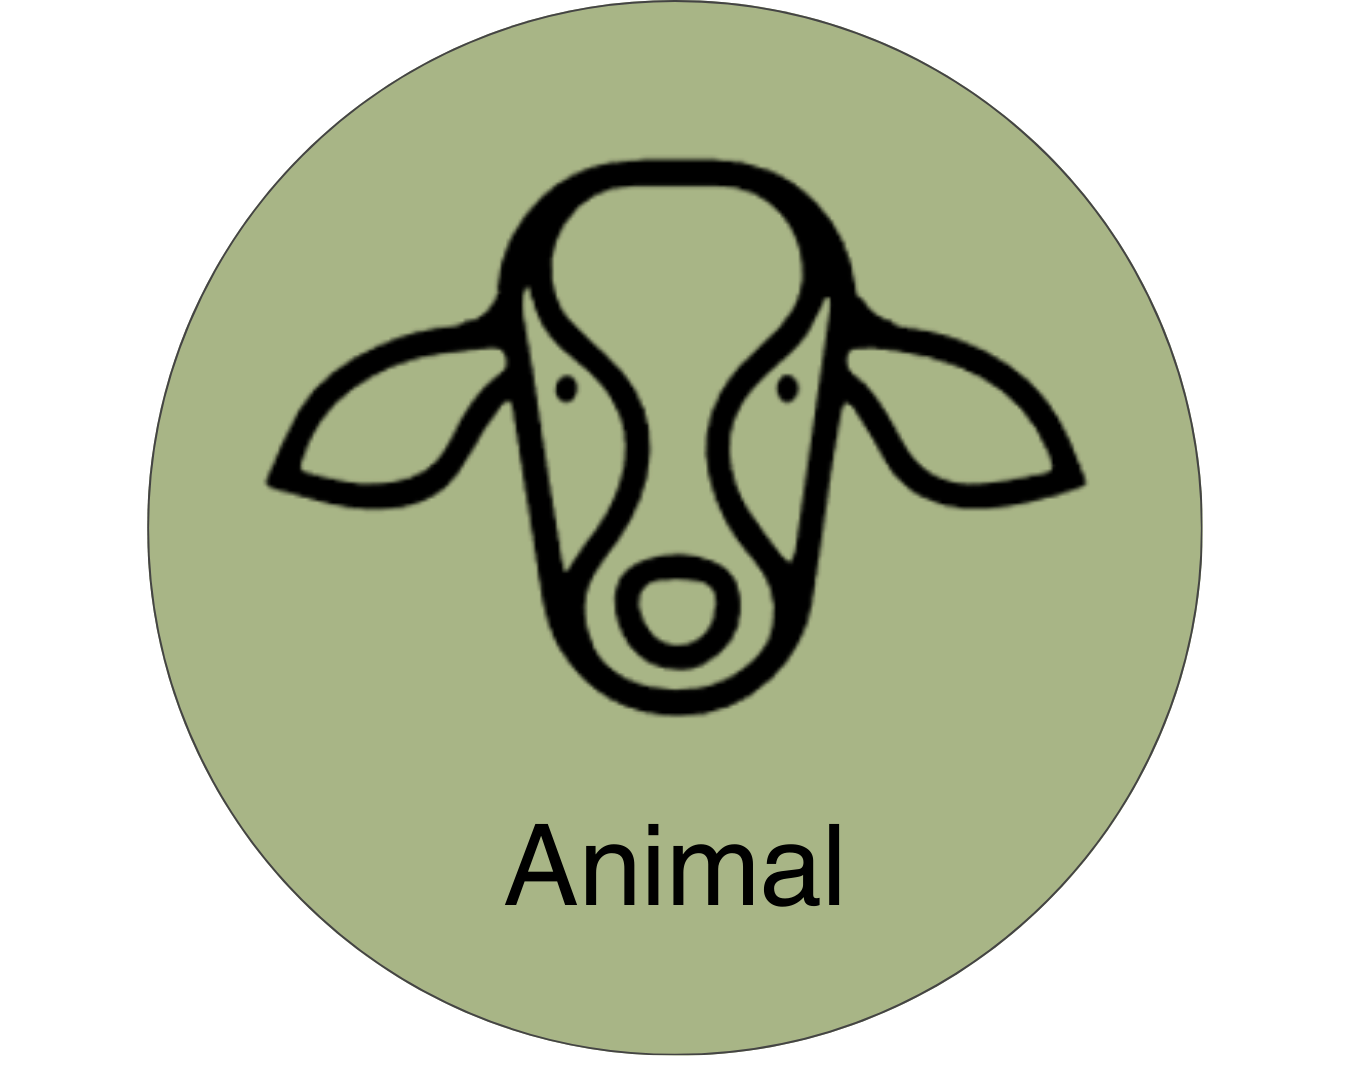
\includegraphics[width=0.35\linewidth,height=\textheight,keepaspectratio]{resources/animal.png}

}

\caption{\label{fig-animal-icon}Animal module icon}

\end{figure}%

\subsection{Example of a Table}\label{example-of-a-table}

\begin{Shaded}
\begin{Highlighting}[]
\PreprocessorTok{|}\NormalTok{ Variable }\PreprocessorTok{|}\NormalTok{ Definition }\PreprocessorTok{|}
\PreprocessorTok{|{-}{-}{-}|{-}{-}{-}|}
\PreprocessorTok{|}\NormalTok{ heiferI\_num }\PreprocessorTok{|}\NormalTok{ Number of Heifer I animals }\PreprocessorTok{|}

\NormalTok{: Example animal inputs \{\#tbl{-}animal{-}inputs\}}


\NormalTok{{-}{-}\textgreater{} The top row of text is your headers and will appear centered and bolded unless otherwise commanded.}
\NormalTok{{-}{-}\textgreater{} The  next row of actual text is what appears in the row with the associated column. Quarto will autowrap to ensure all text fits and is legible. }
\NormalTok{{-}{-}\textgreater{} Be sure to include ..... for between each row}

\NormalTok{{-}{-}\textgreater{} ": Example animal inputs" will appear as the caption. Be as descriptive as possible so that the reader could understand the contents of the table without reading any further text. }
\NormalTok{{-}{-}\textgreater{} \#tbl{-}animal{-}inputs = \#indicates the type of file{-}label{-}for{-}auditing. Though you may label it whatever you want, but be sure that the first part of the label (following the file type) is the module name (e.g. animal, manure, feed, or soilcrop).}
\end{Highlighting}
\end{Shaded}

The above markdown text will appear as it does below:

\begin{longtable}[]{@{}ll@{}}
\caption{Example animal inputs}\label{tbl-animal-inputs}\tabularnewline
\toprule\noalign{}
Variable & Definition \\
\midrule\noalign{}
\endfirsthead
\toprule\noalign{}
Variable & Definition \\
\midrule\noalign{}
\endhead
\bottomrule\noalign{}
\endlastfoot
heiferI\_num & Number of Heifer I animals \\
\end{longtable}

\section{Equation Templates and ID
Logic}\label{equation-templates-and-id-logic}

If you are adding equations, it is important that you continue to use
the ID logic that has been described \ldots{}

\begin{Shaded}
\begin{Highlighting}[]
\NormalTok{$$}
\NormalTok{CBW = MW * 0.06275 \textbackslash{}qquad \textbackslash{}text\{(AN.NRC.2)\}}
\NormalTok{$$ \{\#eq{-}an{-}nrc{-}2\}}

\NormalTok{See }\CommentTok{[}\OtherTok{AN.NRC.2}\CommentTok{](\#eq{-}an{-}nrc{-}2)\textless{}!{-}{-} @eq{-}an{-}nrc{-}2 {-}{-}\textgreater{}}\NormalTok{.}
\end{Highlighting}
\end{Shaded}

\begin{equation}\protect\phantomsection\label{eq-an-nrc-2}{
CBW = MW * 0.06275 \qquad \text{(AN.NRC.50)}
}\end{equation}

See \hyperref[eq-an-nrc-50]{AN.NRC.2}.

\section{Callouts, Recommendations, or
Notes}\label{callouts-recommendations-or-notes}

You may want to emphasize specific notes and annotations. Here is a
helpful tool to do so correctly.

\begin{Shaded}
\begin{Highlighting}[]
\NormalTok{::: \{.callout{-}note\}}
\NormalTok{Callout text goes here}
\NormalTok{:::}
\end{Highlighting}
\end{Shaded}

Your callout will appear the way it does below:

\begin{tcolorbox}[enhanced jigsaw, arc=.35mm, bottomrule=.15mm, bottomtitle=1mm, breakable, colback=white, colbacktitle=quarto-callout-note-color!10!white, colframe=quarto-callout-note-color-frame, coltitle=black, left=2mm, leftrule=.75mm, opacityback=0, opacitybacktitle=0.6, rightrule=.15mm, title=\textcolor{quarto-callout-note-color}{\faInfo}\hspace{0.5em}{Note}, titlerule=0mm, toprule=.15mm, toptitle=1mm]

Note: if only interested in a PDF version of the documentation (no
website version), then the original LaTeX code can still be used and
processed by quarto. For example, the bullet points works as the
original LaTeX or translated into markdown syntax:

\begin{Shaded}
\begin{Highlighting}[]
\InformationTok{\textasciigrave{}\textasciigrave{}\textasciigrave{}\{latex\}}
\InformationTok{\textbackslash{}begin\{itemize\}}
\InformationTok{    \textbackslash{}item first bullet point}
\InformationTok{    \textbackslash{}item second bullet point}
\InformationTok{    \textbackslash{}item ...}
\InformationTok{\textbackslash{}end\{itemize\}}
\InformationTok{\textasciigrave{}\textasciigrave{}\textasciigrave{}}
\end{Highlighting}
\end{Shaded}

\begin{Shaded}
\begin{Highlighting}[]
\InformationTok{\textasciigrave{}\textasciigrave{}\textasciigrave{}\{markdown\}}
\SpecialStringTok{* }\NormalTok{first bullet point}
\SpecialStringTok{* }\NormalTok{second bullet point}
\SpecialStringTok{* }\NormalTok{...}
\InformationTok{\textasciigrave{}\textasciigrave{}\textasciigrave{}}
\end{Highlighting}
\end{Shaded}

\begin{itemize}
\tightlist
\item
  first bullet point
\item
  second bullet point
\item
  \ldots{}
\end{itemize}

but only the markdown works for all document types (html, pdf, word
document, presentations, e-books, etc.).

\end{tcolorbox}

\section{References}\label{references}

Before adding a new reference to ``rufas.bib,'' check the file to ensure
it has not already been added. All references should be listed
alphabetically and then by year (most recent at the top).

If you do need to add a bibliography, the correct structure is below.
Pay special attention to the green text, this formatting is important to
maintain consistentcy because it helps us with our auditing report and
allows us to properly cite in-text.

\begin{Shaded}
\begin{Highlighting}[]
\CommentTok{Journal Articles}
\VariableTok{@article}\NormalTok{\{}\OtherTok{LASTNAME\_YEAR}\NormalTok{,}
  \DataTypeTok{author}\NormalTok{ = \{LASTNAME, FIRSTNAME\},}
  \DataTypeTok{title}\NormalTok{ = \{Title of the article in proper formatting\},}
  \DataTypeTok{journal}\NormalTok{ = \{Journal Title with proper NCBI Abbreviations\},}
  \DataTypeTok{year}\NormalTok{ = \{YEAR PUBLISHED\},}
  \DataTypeTok{volume}\NormalTok{ = \{VOLUME NUMBER\},}
  \DataTypeTok{pages}\NormalTok{ = \{PAGES\}}
\NormalTok{\}}

\CommentTok{Books }

\VariableTok{@book}\NormalTok{\{}\OtherTok{LASTNAME\_YEAR}\NormalTok{,}
  \DataTypeTok{author}\NormalTok{ = \{FIRSTNAME LASTNAME\},}
  \DataTypeTok{title}\NormalTok{ = \{Title of Book Referenced\},}
  \DataTypeTok{publisher}\NormalTok{ = \{Publisher\},}
  \DataTypeTok{year}\NormalTok{ = \{YEAR PUBLISHED\},}
  \DataTypeTok{isbn}\NormalTok{ = \{978{-}3{-}319{-}24277{-}4\}}
\NormalTok{\}}

\CommentTok{Online, Misc, Website (RARE USAGE)}

\VariableTok{@online}\NormalTok{\{}\OtherTok{quarto2024}\NormalTok{,}
  \DataTypeTok{author}\NormalTok{ = \{Posit\},}
  \DataTypeTok{title}\NormalTok{ = \{Quarto Citations Guide\},}
  \DataTypeTok{year}\NormalTok{ = \{2024\},}
  \DataTypeTok{url}\NormalTok{ = \{https://quarto.org/docs/authoring/citations.html\}}
\NormalTok{\}}
\end{Highlighting}
\end{Shaded}

If there are 2 articles with the same author and same year, add the
recommended ``a'' or ``b''
(e.g.~\texttt{bibtex\ @LASTNAME\_YEARa\ vs\ @LASTNAME\_YEARb}) as they
are referenced.

\bookmarksetup{startatroot}

\chapter{Equation examples (from Animal
Documentation)}\label{equation-examples-from-animal-documentation}

\section{Nutrient Requirements of Dairy Cattle (NRC)}\label{sec-nrc}

\textbf{Energy Requirements} For details about the variables included in
each calculation, please refer to the
\href{energy\%20requirements\%20key}{energykey}.

\begin{itemize}
\item
  \textbf{\emph{Maintenance}} - The maintenance requirement is
  calculated based on metabolic body weight (body weight\(^{0.75}\)).

  \ul{Lactating and Dry Cows}

  \begin{equation}\protect\phantomsection\label{eq-nrc-cbw}{
  CBW = MW * 0.06275
  }\end{equation}

  \begin{equation}\protect\phantomsection\label{eq-nrc-cw}{
  CW = {(18 + (DOP - 190) * 0.665) * \left(\frac{CBW}{45}\right), \text{if } DOP > 190.0}
  }\end{equation}

  \emph{Otherwise}

  \begin{equation}\protect\phantomsection\label{eq-nrc-ne-maint}{
  NEmaint = 0.08 \times (BW - CW)^{0.75}
  }\end{equation}
\end{itemize}

\section{Reformatted equations}\label{reformatted-equations}

\ref{eq-nrc-cbw} may be visually improved by using the
\texttt{\textbackslash{}times} LaTeX command:

\begin{equation}\protect\phantomsection\label{eq-nrc-cbw-times}{
CBW = MW \times 0.06275
}\end{equation}

\section{Use alphanumeric equation
labels}\label{use-alphanumeric-equation-labels}

Though Quarto does not allow custom cross-reference labels, you can
include your own non-CR label with the \texttt{\textbackslash{}tag}
LaTeX command. The equation can still be cross-referenceable using a
standard Quarto equation ID.

\begin{equation}\protect\phantomsection\label{eq-an-nrc-2-tagged}{
CBW = MW * 0.06275 \tag{AN.NRC.2}
}\end{equation}

See \ref{eq-an-nrc-2-tagged}.

\section{Other equation Templates}\label{other-equation-templates}

The energy balance is \(E = mc^2\).

\begin{equation}\protect\phantomsection\label{eq-energy}{
E = mc^2
}\end{equation}

See Equation \ref{eq-energy}.

\begin{equation}\protect\phantomsection\label{eq-nutrient-proportion}{
\text{nutrient\_proportion\_to\_be\_removed} =
\min\left(
\frac{\text{mass\_requested\_nutrient}}{\text{manure\_nutrient\_available}},
1
\right)
}\end{equation}

\begin{tcolorbox}[enhanced jigsaw, arc=.35mm, bottomrule=.15mm, bottomtitle=1mm, breakable, colback=white, colbacktitle=quarto-callout-note-color!10!white, colframe=quarto-callout-note-color-frame, coltitle=black, left=2mm, leftrule=.75mm, opacityback=0, opacitybacktitle=0.6, rightrule=.15mm, title=\textcolor{quarto-callout-note-color}{\faInfo}\hspace{0.5em}{Previews and Audits}, titlerule=0mm, toprule=.15mm, toptitle=1mm]

\emph{For preview html}

\begin{Shaded}
\begin{Highlighting}[]
\InformationTok{\textasciigrave{}\textasciigrave{}\textasciigrave{}\{markdown\}}

\NormalTok{quarto preview}

\InformationTok{\textasciigrave{}\textasciigrave{}\textasciigrave{}}
\end{Highlighting}
\end{Shaded}

\emph{For preview pdf}

\begin{Shaded}
\begin{Highlighting}[]
\InformationTok{\textasciigrave{}\textasciigrave{}\textasciigrave{}\{markdown\}}

\NormalTok{quarto render {-}{-}to pdf}

\InformationTok{\textasciigrave{}\textasciigrave{}\textasciigrave{}}
\end{Highlighting}
\end{Shaded}

\emph{For audit review} You can find the output in the quarto-scidoc
folder.

\begin{Shaded}
\begin{Highlighting}[]
\InformationTok{\textasciigrave{}\textasciigrave{}\textasciigrave{}\{markdown\}}

\NormalTok{python quarto\_audit.py}

\InformationTok{\textasciigrave{}\textasciigrave{}\textasciigrave{}}
\end{Highlighting}
\end{Shaded}

\end{tcolorbox}

\bookmarksetup{startatroot}

\chapter{Animal Module}\label{animal-module-1}

\begin{figure}[H]

{\centering 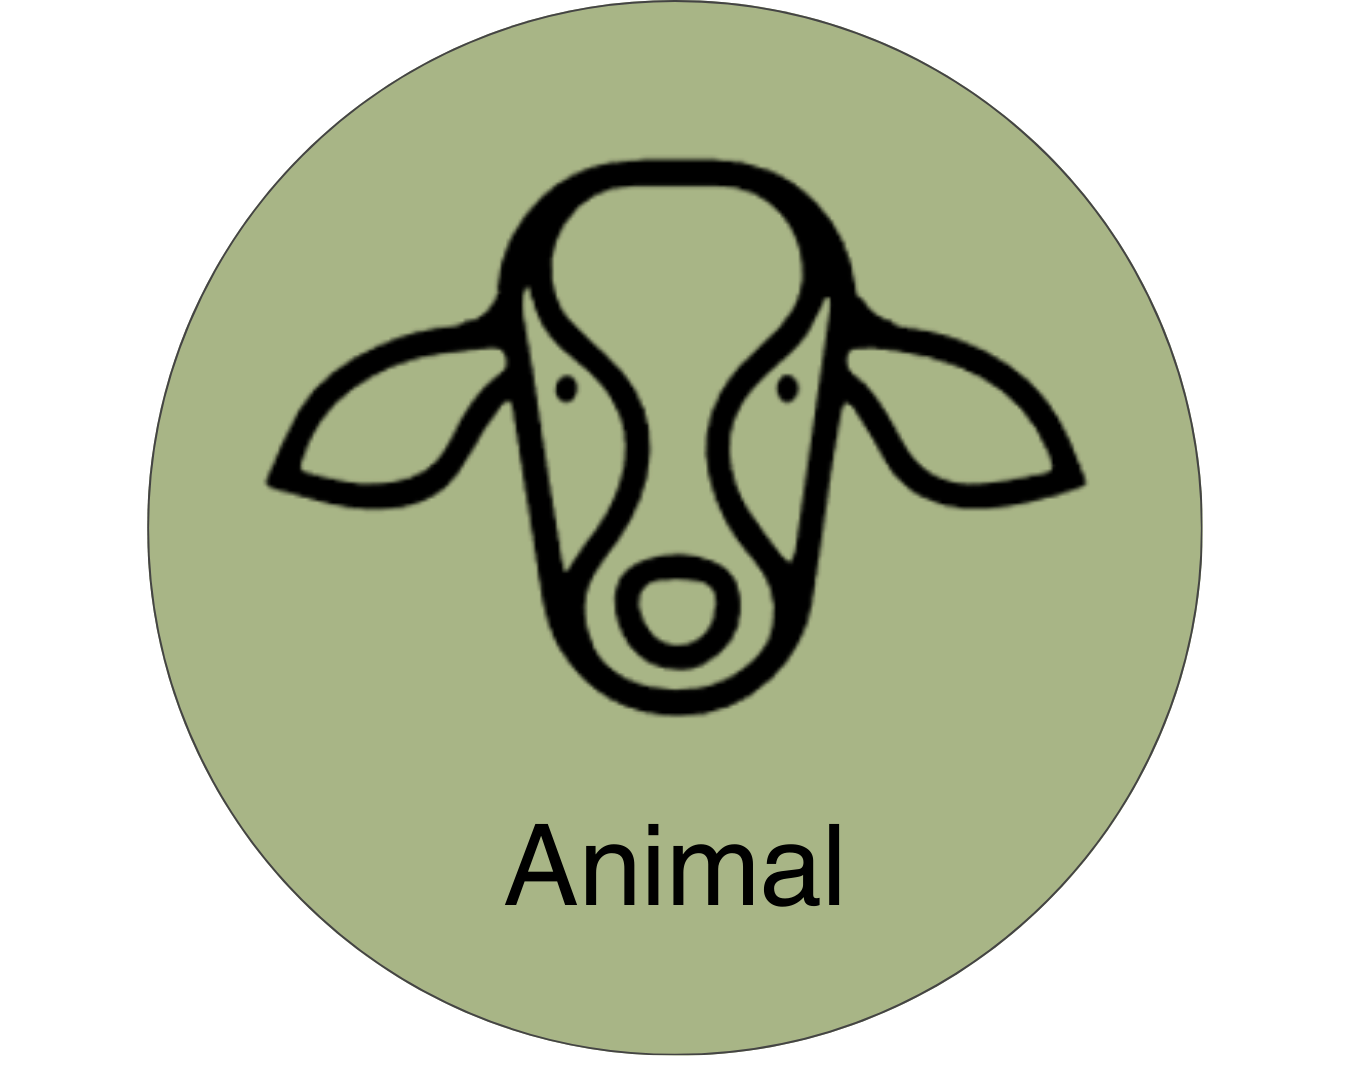
\includegraphics[width=0.35\linewidth,height=\textheight,keepaspectratio]{resources/animal.png}

}

\caption{Animal module icon}

\end{figure}%

\section{Introduction}\label{introduction}

The Animal Module simulates individual animals on a daily basis
throughout each stage of life from birth until removal from the herd. In
addition to the dynamic Monte-Carlo models that determine the occurrence
of events throughout each animal's life, the Animal Module uses
process-based, dynamic models to simulate the following processes:

\begin{itemize}
\tightlist
\item
  Individual animal growth
\item
  Gestation and milk production
\item
  Estimation of nutrient requirements and feed intake
\item
  Enteric emission and manure excretion
\end{itemize}

\subsection{Animal Life Cycle}\label{animal-life-cycle}

The animal life cycle is driven by Monte Carlo stochastic processes that
simulate the growth, production, reproduction, and culling of individual
dairy cattle animals and shares aggregated outcomes with the herd
management sub-module to manage herd dynamics on a daily basis.

The life cycle module represents the variation in animal performance
through the use of Monte Carlo Simulation methods (Reuven and Kroese
2017). Monte Carlo simulation relies on random draws from probability
distributions rather than assigning fixed values. In this model, two
main strategies are used:

\begin{itemize}
\tightlist
\item
  Event-based, in which a random draw from a uniform distribution
  (U(0,1)) is compared to the probability of an event occurring to
  simulate if that event occurs, and
\item
  Population-based, in which a random draw from a known distribution of
  attribute values is assigned to an animal at instantiation.
  Probability distributions used for that purpose are Normal Gaussian or
  Empirical.
\end{itemize}

Each animal within the RuFaS herd progresses through five main life
stages (calf, Heifer I, Heifer II, Heifer III, and Cow) as illustrated
in the figure below.

\begin{itemize}
\tightlist
\item
  Calves progress to Heifer I when their age reaches the user-defined
  input for weaning day
\item
  Heifer I progresses to Heifer II when their age reaches the
  user-defined input for breeding start day
\item
  Heifer II animals that successfully conceive become Heifer III's when
  the number of days left in their pregnancy is equal to the
  user-defined input for prefresh days (default 21)
\item
  When a Heifer III calves, she becomes a Cow for the rest of her life
  on the RuFaS farm
\item
  Cows cycle through lactating and non-lactating phases until they are
  removed from the herd due to a failure to conceive or a user-provided
  probability for sale or death within each parity (lactation).
\end{itemize}

When a HeiferIII or Cow reaches full gestation length, they start
lactating and a new calf object is created. The calf is assigned a
birthweight according to a user-informed random distribution. All male
calves are recorded and removed from the farm on day 1 of their life.
Female calves either remain on the farm or are sold on day 1, determined
by an event-based Monte Carlo method informed by the user-defined
percent of female calves that are kept.

\section{Herd-level Processes and
Management}\label{herd-level-processes-and-management}

\section{Herd Initialization}\label{herd-initialization}

\begin{tcolorbox}[enhanced jigsaw, arc=.35mm, bottomrule=.15mm, bottomtitle=1mm, breakable, colback=white, colbacktitle=quarto-callout-note-color!10!white, colframe=quarto-callout-note-color-frame, coltitle=black, left=2mm, leftrule=.75mm, opacityback=0, opacitybacktitle=0.6, rightrule=.15mm, title=\textcolor{quarto-callout-note-color}{\faInfo}\hspace{0.5em}{Note}, titlerule=0mm, toprule=.15mm, toptitle=1mm]

In RuFaS code, the term ``herd initialization'' is used to refer to both
the process of generating an animal population file and of selecting
from that population to create a specific herd at the start of a
simulation. In this doc, those two processes will be differentiated by
calling them ``Generation'' and ``Selection'', respectively.

``Animal population'' can refer to both groups of animals (the pool of
animals generated, and the herd of animals selected). In the code, the
population is sometimes referred to as ``pre\_animal\_population'' and
``post\_animal\_population'' to differentiate whether the specified
group of animals exists before or after the random selection of
individuals to create a herd.

\end{tcolorbox}

\subsection{Introduction to Herd
Initialization}\label{introduction-to-herd-initialization}

Every simulation begins with a herd consisting of calves, heifers, and
dry and lactating cows. This herd comes to be through a two-step
process:

\begin{itemize}
\tightlist
\item
  A population of animals is generated through simulation or loaded from
  data (pre-animal-population). The animals in that herd should reflect
  the attributes of animals in the herd to be modeled.
\item
  Animals are randomly selected with replacement from the
  pre-animal-population to be in the initial herd, based on group
  numbers and characteristics that reflect the distribution of animals
  within the herd being modeled. Note that the animals in the herd on
  day one will have attributes of the pre-animal-population and may
  deviate from the desired herd to be modeled.
\end{itemize}

For the rest of the simulation, animals enter the herd through birth as
newborn calves or purchased replacements (heiferIII's).

\begin{longtable}[]{@{}
  >{\raggedright\arraybackslash}p{(\linewidth - 4\tabcolsep) * \real{0.2875}}
  >{\raggedright\arraybackslash}p{(\linewidth - 4\tabcolsep) * \real{0.3500}}
  >{\raggedright\arraybackslash}p{(\linewidth - 4\tabcolsep) * \real{0.3500}}@{}}
\caption{Overview of the distinct phases by which animals are created
and introduced to the herd.}\label{tbl-animal-simulation}\tabularnewline
\toprule\noalign{}
\begin{minipage}[b]{\linewidth}\raggedright
Before Simulation
\end{minipage} & \begin{minipage}[b]{\linewidth}\raggedright
Simulation Initiation
\end{minipage} & \begin{minipage}[b]{\linewidth}\raggedright
During the Simulation
\end{minipage} \\
\midrule\noalign{}
\endfirsthead
\toprule\noalign{}
\begin{minipage}[b]{\linewidth}\raggedright
Before Simulation
\end{minipage} & \begin{minipage}[b]{\linewidth}\raggedright
Simulation Initiation
\end{minipage} & \begin{minipage}[b]{\linewidth}\raggedright
During the Simulation
\end{minipage} \\
\midrule\noalign{}
\endhead
\bottomrule\noalign{}
\endlastfoot
Generate (simulate) or load an Animal Population file (pre-animal-
population).

The animals present at the start of the simulation, and those available
in the replacement market, are drawn from this file. & Herd is
established by random selection of animals from the Animal Population to
match the user-specified group sizes and age/stage distribution (post-
animal-population).

Management attributes, including lactation- curve parameters, are
assigned as each animal enters the herd. & New animals enter via (a)
birth or (b) purchase\textbar{} of heifers from the \textbar{}
replacement market.

Purchased animals inherit\textbar{} two attributes from the \textbar{}
population file, \textbar{} - Breed \textbar{} - Mature bodyweight
\textbar{} \\
\end{longtable}

\textbf{Relevant Inputs}

\begin{longtable}[]{@{}
  >{\raggedright\arraybackslash}p{(\linewidth - 8\tabcolsep) * \real{0.2000}}
  >{\raggedright\arraybackslash}p{(\linewidth - 8\tabcolsep) * \real{0.2000}}
  >{\raggedright\arraybackslash}p{(\linewidth - 8\tabcolsep) * \real{0.2000}}
  >{\raggedright\arraybackslash}p{(\linewidth - 8\tabcolsep) * \real{0.2000}}
  >{\raggedright\arraybackslash}p{(\linewidth - 8\tabcolsep) * \real{0.2000}}@{}}
\caption{User inputs in the animal input file that influence the
generation of the Animal Population (pre-animal-population). The inputs
of this table are found in the Herd Initialization
Section.}\label{tbl-animal-herd-inputs}\tabularnewline
\toprule\noalign{}
\begin{minipage}[b]{\linewidth}\raggedright
Variable
\end{minipage} & \begin{minipage}[b]{\linewidth}\raggedright
Definition
\end{minipage} & \begin{minipage}[b]{\linewidth}\raggedright
Default
\end{minipage} & \begin{minipage}[b]{\linewidth}\raggedright
Min
\end{minipage} & \begin{minipage}[b]{\linewidth}\raggedright
Max
\end{minipage} \\
\midrule\noalign{}
\endfirsthead
\toprule\noalign{}
\begin{minipage}[b]{\linewidth}\raggedright
Variable
\end{minipage} & \begin{minipage}[b]{\linewidth}\raggedright
Definition
\end{minipage} & \begin{minipage}[b]{\linewidth}\raggedright
Default
\end{minipage} & \begin{minipage}[b]{\linewidth}\raggedright
Min
\end{minipage} & \begin{minipage}[b]{\linewidth}\raggedright
Max
\end{minipage} \\
\midrule\noalign{}
\endhead
\bottomrule\noalign{}
\endlastfoot
Initial\_animal\_num & The initial number of animals that serve as a
starting point for the population generation simulation & 10000 & 0 &
- \\
Simulation\_days & The number of days to simulate for the population
generation simulation & 5000 & 0 & - \\
Calf\_num & Number of Calves (head) -- The initial number of pre-weaned
calves & 8 & 2 & -- \\
HeiferI\_num & Number of HeiferI animals (head) -- The initial number of
heifers that are weaned but not yet bred & 44 & 2 & -- \\
HeiferII\_num & Number of HeiferII animals (head) -- The initial number
of heifers that are either eligible for breeding (based on user-inputted
Breeding Start Day for heifers), or in early pregnancy & 38 & 2 & -- \\
HeiferIII\_num\_springers & Number of HeiferIII animals (head) -- The
initial number of close-up heifers (within the user-defined close-up
period, e.g., Prefresh Day) & 5 & 2 & -- \\
Cow\_num & Number of Cows (head) -- The initial number of dry and
lactating cows & 100 & 6 & -- \\
Replace\_num & replacements (head) -- Number of replacement animals
available in the replacement market & 5000 & 50 & -- \\
Lactating\_fraction & Fraction of cows that are lactating. Used during
herd initialization & 0.8356 & 0 & 1 \\
Parity\_fractions: 1, 2, 3, 4, 5 & Fractions of the milking animal
population that are parity 1, 2, 3, 4, and 5+. The sum must equal 1.0 &
0.36, 0.26, 0.18, 0.11, 0.09 & 0 & 1 \\
\end{longtable}

\textbf{Relevant Outputs}

After the animals have been selected from the animal population to
create the initial herd, a summary of the Population (pre-selection
pool, aka pre-animal-population) and of the Initial herd (selected
animals, aka post-animal-population) is provided to the output manager.

Class and function:
AnimalModuleReporter.report\_animal\_population\_statistics

Output variables: - .population\_\{\ldots\} - .initial\_\{\ldots\}

\{\ldots\} includes: breed, number of animals of each class (calf,
heiferI, heiferII, heiferIII, cow), number of cows by parity and
lactation status, average age of animals within each class, distribution
of age of animals within each class, average body weight of animals
within each class, average cow days in milk, days in preg, parity, and
calving interval.

\subsection{Methodology}\label{methodology}

When a simulation begins, the HerdFactory class generates or loads the
pre-animal-population, from which it selects and compiles the
post-animal-population with an appropriate distribution of animal ages
and stages to serve as the starting herd for simulation.

\textbf{Designation of an Animal Population}

\begin{itemize}
\tightlist
\item
  Option 1: Creating a new Animal Population An animal population can be
  generated as a stand-alone simulation task that creates and saves a
  pre-animal-population file as the output based on the user Animal
  Module inputs. Or, the animal population can be generated as the first
  step of a regular simulation task which then uses that generated
  pre-animal-population to select from and create the
  post-animal-population to use for the subsequent herd simulation. See
  the documentation about Task Manager for more information about how to
  generate a new pre-animal-population.
\end{itemize}

The \_generate\_animals() method creates the pre\_animal\_population,
with the option to save those animals to file at the end of the
generation process.

Calves are created according to the number specified by the user
(initial\_animal\_num), some are sold based on user inputs, and those
remaining proceed through select daily updates (growth, reproduction,
milk, and transition through the appropriate life stages) for the
user-specified number of days (simulation\_days). The simulation occurs
similarly to the regular life cycle simulation process, but with an
extended period and large number of animals. There are a few notable
distinctions:

\begin{itemize}
\tightlist
\item
  After 3000 days of simulation (specified in animal\_constants), a copy
  of each heiferIII is saved to the replacement herd. The copy is made
  on the day when she is ready to transition to a lactating cow (ready
  to give birth), so that when the copy enters the herd as a purchased
  heiferIII during the actual simulation, she will give birth the very
  next day.
\item
  If a cow has made it to parity six without being culled, she is
  removed from the herd. (The maximum parity of cows kept in the
  generated herd is five).
\end{itemize}

After the simulation\_days number of days, the full herd contains a
mixture of calves, heifers, cows, and replacements. The core status
information and life history of each animal are either saved to file or
passed for random sampling to create the post-animal-population.

\begin{itemize}
\tightlist
\item
  Option 2: Point to an existing Animal Population Alternatively, the
  pre-animal-population will be loaded from a specified Animal
  Population input file consisting of calf, heifer, cow, and replacement
  objects.
\end{itemize}

\emph{Herd Selection} The \_random\_sample\_with\_replacement() method
selects animals from each of the following groups: calf, heiferI,
heiferII, heiferIII, replacement, lactating cows by parity for parities
1-5, and dry cows by parity for parities 1-5.

Animals are sampled randomly with replacement from the
pre-animal-population according to the numbers, parity fractions, and
milking cow fraction specified in the animal input file. The resulting
list of animals is returned as the post-animal-population and summaries
of the pre- and post-animal-populations are reported to the output
manager.

\section{Pens and Animal Grouping}\label{pens-and-animal-grouping}

\subsection{Introduction to Grouping}\label{introduction-to-grouping}

All animals in RuFaS are assigned to a pen which is used to summarize
nutrient requirements for diet formulation and feeding, aggregate
enteric methane and manure excretions for reporting and passage to the
Manure Module. Each pen tracks and updates daily a list of animals in
the pen, the stocking density, the average nutrient requirement of the
animals in the pen, the ration being fed to that pen, the manure
excreted, and the methane emitted. In addition, constant attributes of
each pen include the type of pen it is (freestall, tiestall, open lot,
compost bedded pack barn), the type of animals that can be in that pen,
the number stalls, the manure management practices associated with that
pen, and the distance to the milking parlor for lactating cows. Each day
after the HerdManager has updated the status of each animal and
determined which animals need to be bought or sold, the animals are
added and removed from pens as needed.

\textbf{Relevant Inputs}

\begin{longtable}[]{@{}
  >{\raggedright\arraybackslash}p{(\linewidth - 8\tabcolsep) * \real{0.2857}}
  >{\raggedright\arraybackslash}p{(\linewidth - 8\tabcolsep) * \real{0.3839}}
  >{\raggedright\arraybackslash}p{(\linewidth - 8\tabcolsep) * \real{0.0982}}
  >{\raggedright\arraybackslash}p{(\linewidth - 8\tabcolsep) * \real{0.0625}}
  >{\raggedright\arraybackslash}p{(\linewidth - 8\tabcolsep) * \real{0.1429}}@{}}
\caption{User inputs in the animal input file that influence pen
grouping. The user must define at least 3 pens and for each pen, key
inputs are outlined here.}\label{tbl-animal-grp-inputs}\tabularnewline
\toprule\noalign{}
\begin{minipage}[b]{\linewidth}\raggedright
Variable
\end{minipage} & \begin{minipage}[b]{\linewidth}\raggedright
Definition
\end{minipage} & \begin{minipage}[b]{\linewidth}\raggedright
Default
\end{minipage} & \begin{minipage}[b]{\linewidth}\raggedright
Min
\end{minipage} & \begin{minipage}[b]{\linewidth}\raggedright
Max
\end{minipage} \\
\midrule\noalign{}
\endfirsthead
\toprule\noalign{}
\begin{minipage}[b]{\linewidth}\raggedright
Variable
\end{minipage} & \begin{minipage}[b]{\linewidth}\raggedright
Definition
\end{minipage} & \begin{minipage}[b]{\linewidth}\raggedright
Default
\end{minipage} & \begin{minipage}[b]{\linewidth}\raggedright
Min
\end{minipage} & \begin{minipage}[b]{\linewidth}\raggedright
Max
\end{minipage} \\
\midrule\noalign{}
\endhead
\bottomrule\noalign{}
\endlastfoot
id & The index of the pen & NA & 0 & NA \\
pen\_name & The name or identifier of a given pen & NA & & \\
animal\_combination & The valid combinations of animal types that can be
in a pen. CALF = Calves; GROWING = HeiferI's and HeiferII's; CLOSE\_UP =
HeiferIII's and Dry Cows; LAC\_COWS = Lactating Cows & & & CALF,
GROWING, CLOSE\_UP, LAC\_COWS \\
vertical\_dist\_to\_milking\_ parlor & The elevation gain (in meters)
between the pen and the milking parlor & 0.1 & 0 & NA \\
horizontal\_dist\_to\_milking\_ parlor & The distance (in meters)
between the pen and the milking parlor & 10 & 0 & NA \\
number\_of\_stalls & The number of stalls in the pen & 1000 & 0 & NA \\
pen\_type & The type of pen (freestall, tiestall, open lot, compost
bedded pack barn) & freestall & & freestall, tiestall, open lot, compost
bedded pack barn \\
max\_stocking\_density & The maximum ratio of the number of animals in
the pen to the number of stalls in the pen & 1.2 & 0.5 & 5 \\
manure\_management\_ scenario\_id & The ID number of the manure
management practices that are used for this pen (scenarios are defined
in manure management schema) & 0 & 0 & NA \\
\end{longtable}

\textbf{Relevant Outputs}

\begin{itemize}
\item
  \begin{itemize}
  \tightlist
  \item
    \textbf{number\_of\_animals\_in\_pen\_{[}id{]}\_{[}AnimalCombination{]}}
    - reports the number of animals in each pen each day.
  \end{itemize}
\item
  \textbf{ration\_per\_animals\_for\_pen\_{[}id{]}\_{[}AnimalCombination{]}}
  - reports average dry matter intake of an animal in the pen at the
  time of the ration formulation.
\item
  \textbf{ration\_per\_animals\_for\_pen\_{[}id{]}\_{[}AnimalCombination{]}.{[}RUFAS\_feed\_id{]}}
  - reports the amount of each feed that is delivered per animal in the
  pen
\item
  \textbf{ration\_nutrient\_amount\_for\_pen\_{[}AnimalCombination{]}.{[}nutrient{]}}
  - is reporting the amount of each of the following nutrients that is
  provided by the ration per animal in the pen (all reported in
  kilograms unless otherwise indicated)
\end{itemize}

\subsection{Methodology}\label{methodology-1}

\textbf{Animal Grouping} To translate from the AnimalTypes needed to
track an animal's life stages and the combinations of animals that are
allowed to be grouped into a single pen, a new variable called
AnimalCombination is created that combines some AnimalTypes to
facilitate sorting into pens. The AnimalCombination class is defined in
enums.py and includes the following mapping from AnimalTypes to
AnimalCombinations:

\begin{longtable}[]{@{}ll@{}}
\caption{Summary of animal types and their grouping included in this
module.}\label{tbl-animal-grp-inputs}\tabularnewline
\toprule\noalign{}
Animal Combination & Animal Type \\
\midrule\noalign{}
\endfirsthead
\toprule\noalign{}
Animal Combination & Animal Type \\
\midrule\noalign{}
\endhead
\bottomrule\noalign{}
\endlastfoot
CALF & Calves \\
GROWING & Heifer I and Heifer II \\
CLOSE\_UP & Heifer III and Non-lactating Cows \\
LAC\_COW & Lactating Cows \\
\end{longtable}

Currently there are only two options for assigning AnimalCombinations to
pens.

\begin{itemize}
\item
  \emph{Option 1} The first and most commonly used option for grouping
  animals is to assign one AnimalCombination to each pen such that there
  is at least one pen for the 4 AnimalCombinations: CALF, GROWING,
  CLOSE\_UP, and LAC\_COW.
\item
  \emph{Option 2} In some cases, and especially in very small farms, a
  user might wish to represent a scenario where all growing animals,
  pregnant heifers, and non-lactating cows are housed together. In this
  case, there is an option to have a pen that houses both GROWING and
  CLOSE\_UP animals such that the there is at least one pen with each of
  the 3 AnimalCombination inputs: CALF, GROWING\_AND\_CLOSE\_UP, and
  LAC\_COW.
\end{itemize}

Pen Sizing: Due to oscillations in the exact number of animals in each
animal type, it is strongly recommended that the stocking density is at
least 120\% of the expected number of animals in each pen.

Class: \emph{Pens} are inare initiated from the Pen class by the
HerdManager at the beginning of the simulation and, if needed, an
additional pen is created to accommodate animals if the animal numbers
have exceeded the max stocking density.

\begin{tcolorbox}[enhanced jigsaw, arc=.35mm, bottomrule=.15mm, bottomtitle=1mm, breakable, colback=white, colbacktitle=quarto-callout-note-color!10!white, colframe=quarto-callout-note-color-frame, coltitle=black, left=2mm, leftrule=.75mm, opacityback=0, opacitybacktitle=0.6, rightrule=.15mm, title=\textcolor{quarto-callout-note-color}{\faInfo}\hspace{0.5em}{Note}, titlerule=0mm, toprule=.15mm, toptitle=1mm]

\textbf{Remove\_animals\_by\_ids} - This function is called when the
HerdManager calls for: remove\_animal\_from\_pen\_and\_id\_map.

It is pen specific and removes the animal from the pen and the animal ID
from the animal ID map that tracks the animals in the pen.

**\_add\_new\_animals** - This function is called by Pen.update\_animals
which is in turn called by
HerdManager.\_add\_animal\_to\_pen\_and\_id\_map. Thus, when HerdManager
initiates addition of animals to each pen, this function executes the
addition of those animals \_animal\_nutritional\_requirements

\end{tcolorbox}

\section{Ration Formulation}\label{ration-formulation}

The diet recipes in RuFaS are either formulated through least-cost
formulation (Li et al. 2022) or provided by the user for each of 4
animal categories (calves, growing heifers, dry and close-up cows, and
lactating cows). The composition of the available feeds are provided by
a feed library that was adapted from the (National Academies of
Sciences, Engineering, and Medicine 2021). The amount of feed required
by the farm is tracked by pen and multiple pens of each animal category
can be simulated; however, at this time, the RuFaS model can only accept
1 user-defined diet per animal category even if there are multiple
simulated pens for that animal category.

In practice, animal feeding on dairy farms is a constantly evolving
process that responds to fluctuations in feed availability, animal
requirements and responses, and management goals. Although the feed
delivery algorithms will make small modifications to the diet recipe in
response to animal nutrient requirements and adjust the total amount of
feed delivered based on the number of animals and their requirements,
the diversity and degree of fluctuation in the diets is less than what
is expected on a commercial dairy. The RuFaS feed library can also be
modified or expanded on by changing the compositions of the existing
feeds or by adding new feeds.

Regardless of whether or not a user chooses to provide their own ration
or have RuFaS build and feed a ration optimized for least-cost, RuFaS
needs a set of ingredients to work from. The RuFaS feed library should
be consulted for the full list of ingredients and ingredients that are
in both the NASEM and NRC libraries can be used. Users interested in
feeding a ration that they define, need to provide a list of ingredients
and their relative \% dry matter intake for each animal class
(pre-weaned calves, growing heifers, close-up animals, and lactating
cows).

If a user would like RuFaS to use the list of ingredients to formulate a
least-cost ration, it is imperative that proper costs are inputted for
each ingredient listed, but the \% dry matter intake in the user defined
ration percentages does not need to be included. Feed costs need to be
entered in kg/DM. RuFaS will then use all the ingredients available
(based on costs and inventory available if the feed is homegrown) to
create a ration that meets the nutritional requirements of the animal
class and is cost-optimized.

\begin{tcolorbox}[enhanced jigsaw, arc=.35mm, bottomrule=.15mm, bottomtitle=1mm, breakable, colback=white, colbacktitle=quarto-callout-note-color!10!white, colframe=quarto-callout-note-color-frame, coltitle=black, left=2mm, leftrule=.75mm, opacityback=0, opacitybacktitle=0.6, rightrule=.15mm, title=\textcolor{quarto-callout-note-color}{\faInfo}\hspace{0.5em}{Note}, titlerule=0mm, toprule=.15mm, toptitle=1mm]

For the time being, only one set of feeds and ration formula can be
provided for each animal class.

\end{tcolorbox}

\subsection{Energy and Nutrition
Requirements}\label{energy-and-nutrition-requirements}

\textbf{NRC: Calculating Nutrient Requirements of Dairy Cattle}

Below are the calculations utilized based on the energy and nutrient
requirements of dairy cattle as reported by the NRC and more recently
the NASEM National Research Council (2001), National Academies of
Sciences, Engineering, and Medicine (2021).

Calculations are included for the following requirement categories:

\begin{itemize}
\tightlist
\item
  Energy (Maintenance, Activity, Growth, Pregnancy, Lactation)
\item
  Protein (Maintenance, Growth, Pregnancy, Lactation)
\item
  Minerals (Maintenance, Growth, Pregnancy, Lactation)
\item
  Dry Matter Intake
\item
  Amino Acids (NASEM only)
\end{itemize}

Where appropriate, requirement calculations are differentiated by animal
age and reproductive status.

\subsection{Nutrient Requirements of Dairy Cattle
(NRC)}\label{nutrient-requirements-of-dairy-cattle-nrc}

\textbf{Energy Requirements} For details about the variables included in
each calculation, please refer to tbl-energy-req for a full list.

\emph{Maintenance}The maintenance requirement is calculated based on
metabolic body weight (body weight\(^{0.75}\)).

\subsection{Examples of Equations}\label{examples-of-equations}

\begin{equation}\protect\phantomsection\label{eq-an-nrc-2}{
CBW = MW * 0.06275 \qquad \text{(AN.NRC.2)}
}\end{equation}

\begin{equation}\protect\phantomsection\label{eq-an-nrc-3}{
CBW = MW * 0.06275 \qquad \text{(AN.NRC.3)}
}\end{equation}

\begin{equation}\protect\phantomsection\label{eq-an-nrc-4}{
CBW = MW * 0.06275 \qquad \text{(AN.NRC.4)}
}\end{equation}

\begin{equation}\protect\phantomsection\label{eq-an-nrc-5}{
CBW = MW * 0.06275 \qquad \text{(AN.NRC.5)}
}\end{equation}

\begin{equation}\protect\phantomsection\label{eq-an-nrc-1}{
CBW = MW * 0.06275 \qquad \text{(AN.NRC.1)}
}\end{equation}

\begin{equation}\protect\phantomsection\label{eq-an-nrc-6}{
CBW = MW * 0.06275 \qquad \text{(AN.NRC.6)}
}\end{equation}

See \ref{eq-an-nrc-2}.

\bookmarksetup{startatroot}

\chapter{Manure Module}\label{manure-module-1}

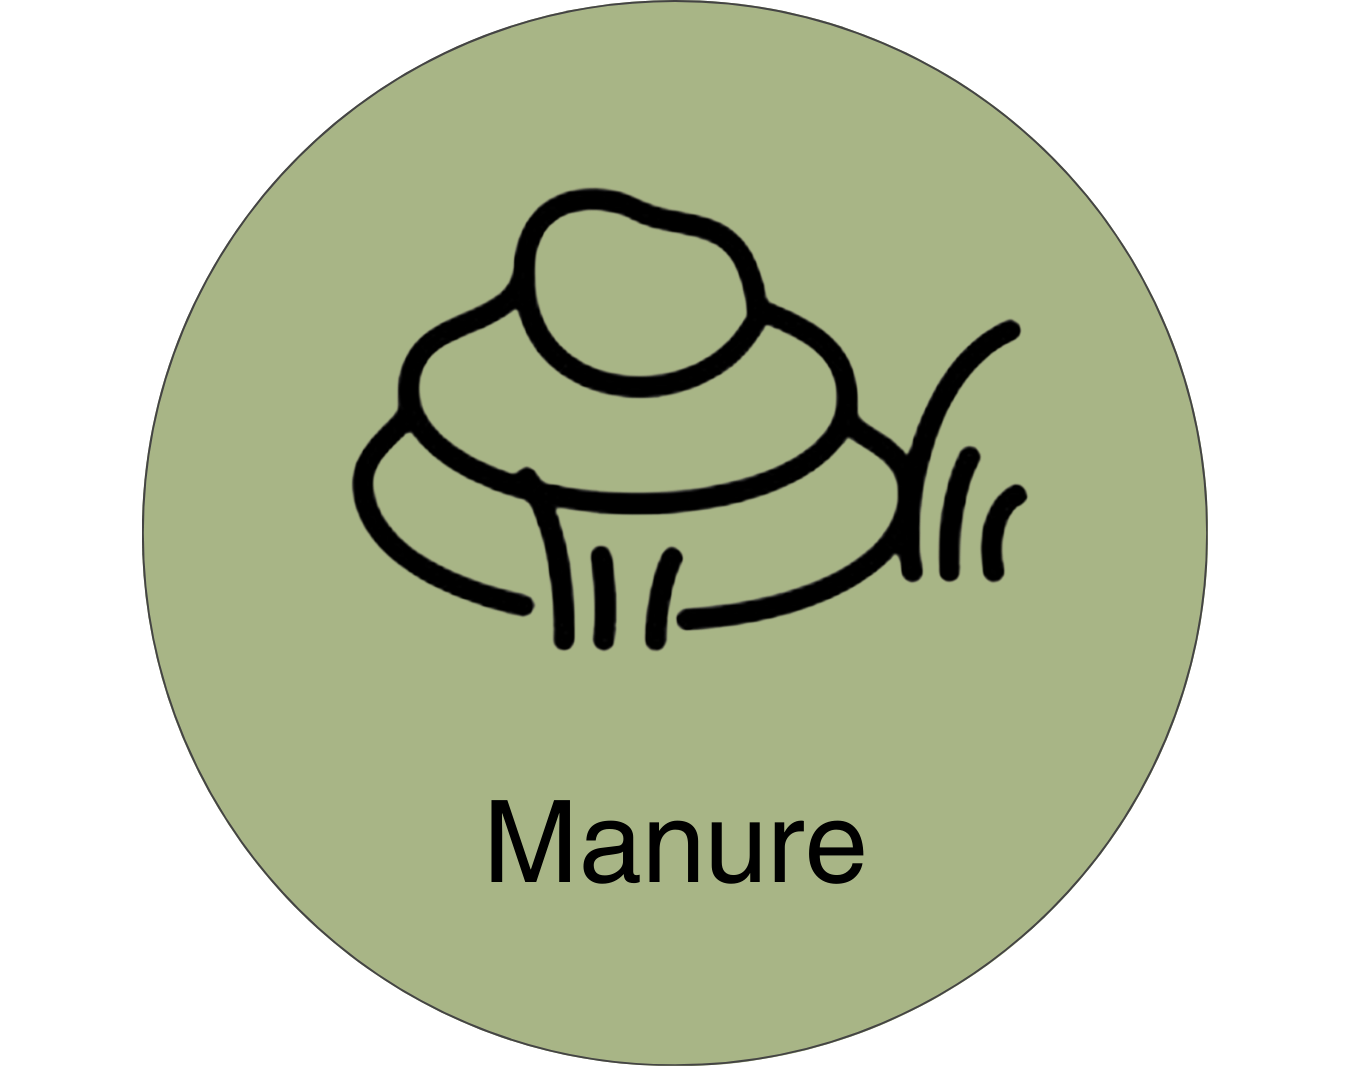
\includegraphics[width=1.45833in,height=\textheight,keepaspectratio]{resources/manure.png}

\section{Introduction}\label{introduction-1}

\subsection{Example of a Figure}\label{example-of-a-figure-1}

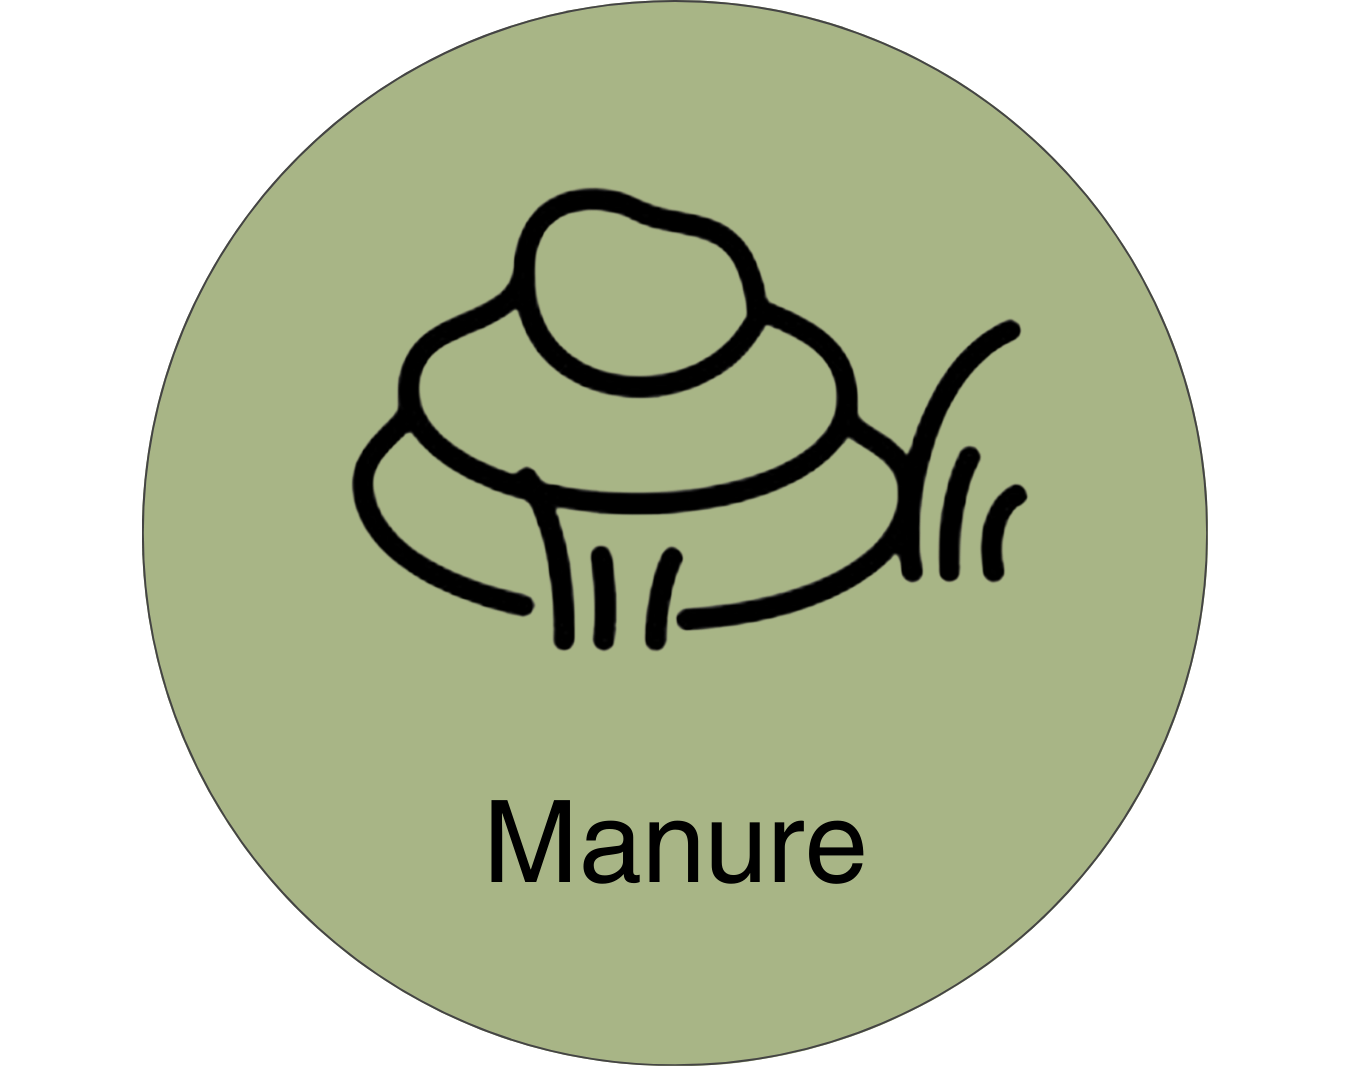
\includegraphics[width=0.5\linewidth,height=\textheight,keepaspectratio]{resources/manure.png}

\subsection{Example of a Table}\label{example-of-a-table-1}

\begin{longtable}[]{@{}ll@{}}
\caption{Example animal inputs}\label{tbl-animal-inputs}\tabularnewline
\toprule\noalign{}
Variable & Definition \\
\midrule\noalign{}
\endfirsthead
\toprule\noalign{}
Variable & Definition \\
\midrule\noalign{}
\endhead
\bottomrule\noalign{}
\endlastfoot
heiferI\_num & Number of Heifer I animals \\
\end{longtable}

\protect\phantomsection\label{refs}
\begin{CSLReferences}{1}{1}
\bibitem[\citeproctext]{ref-Li_2022}
Li, M., G. J. M. Rosa, K. F. Reed, and V. E. Cabrera. 2022.
{``Investigating the Effect of Temporal, Geographic, and Management
Factors on US Holstein Lactation Curve Parameters.''} \emph{J Dairy Sci}
105 (9): 7525--38.

\bibitem[\citeproctext]{ref-nrc_2021}
National Academies of Sciences, Engineering, and Medicine. 2021.
\emph{Nutrient Requirements of Dairy Cattle: Eighth Revised Edition}.
The National Academies Press.

\bibitem[\citeproctext]{ref-nrc_2001}
National Research Council. 2001. \emph{Nutrient Requirements of Dairy
Cattle}. National Academies Press.

\bibitem[\citeproctext]{ref-reuven_2017}
Reuven, Y. R., and D. P. Kroese. 2017. \emph{Simulation and the Monte
Carlo Method. In: Wiley Series in Probability and Statistics}. John
Wiley; Sons Inc.

\end{CSLReferences}


\backmatter


\end{document}
